\section{Understanding Dependency Trees}


Software defines dependencies typically by specifying packages directly
consumed by the software in the build instructions.  These are referred to as
\textit{direct dependencies}.  Each direct dependency may also have
dependencies; dependees of dependencies are referred to as 
\textit{transitive dependencies}.  Each dependency of software can be an
internally developed private package or a publicly available open source package.
\footnote{Commercially developed, closed-source third-party packages are grouped into the
category of open source packages for ease of explanation.}
Figure \ref{fig:dependency_tree} shows an example of a dependency tree.

The dependency tree can have a varying depth depending on the composition
of all dependencies.  If one to review the dependency tree of Hadoop, for
example, a very deep dependency tree with a large variety of packages and
licenses would be observed.  The red boxes in Figure \ref{fig:dependency_tree}
show packages that were detected as having known vulnerabilities.

\begin{figure}[h]
    \caption{Example Dependency Tree}
    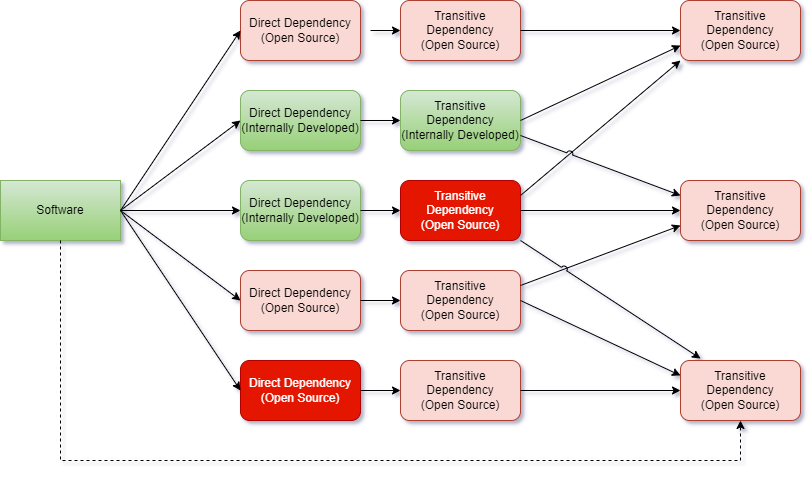
\includegraphics[width=\textwidth]{graphics/dependency_tree.png}
    \label{fig:dependency_tree}
\end{figure}


\subsection{How Detection of Vulnerable Dependencies Can Fail}\label{sec:missing_vulnerable_dependencies}


\subsubsection{Dependency Resolution Happy Path}

One of the potentially vulnerable packages in Figure \ref{fig:dependency_tree} 
is an open source direct dependency of the software.  The detection in this
case is very simple since the dependency is specifically referenced in
the software's build script.  The package is open source, making it well known
and generally available for dependency resolution. Provided the tooling that
can resolve the dependency and a network path to the public repository
is available, the dependency can be resolved.


\subsubsection{Unavailable Private Packages}

The other potentially vulnerable package exhibited in Figure 
\ref{fig:dependency_tree} is a transitive dependency of an internally 
developed direct dependency. A prerequisite of discovering a potentially 
vulnerable package that is a dependee of an internally developed package
is that the internally developed package is available at the time of 
dependency resolution.  

It is often the case that an 
internally developed package is not publicly
available; private packages are typically available through private
package repositories hosted on the organizations internal network.
If that private package repository is not accessible over the network,
the private package and its transitive dependencies will not be available.
The challenges presented in detecting vulnerabilities 
in transitive dependencies of private packages are discussed in detail
in Section \ref{sec:execution_environment}.

\subsubsection{Proper Tooling is Unavailable or Misconfigured}

If the tools required to perform a dependency resolution are not available,
it is apparent that the dependency resolution will fail.  Along with
having the correct tools available, the tools need to be correctly configured.
For example, if a private package repository requires login credentials, 
the dependency resolution will fail unless the tooling configuration provides
those login credentials.

\subsubsection{Improperly Defined Direct Dependencies}

Figure \ref{fig:dependency_tree} depicts a dashed line from the software to a
transitive dependency.  When developers are writing software, it is often
possible to reference packages via namespace.  If a referenced package happens to be
pulled in as a node on the dependency tree below a direct dependency, the
developer may see that a compile and execution works due to the dependency
being resolved as part of the build order.  Since the dependency
is referenced directly in the software, it should be defined as a direct
dependency.  Software can exist and build for years without anyone ever realizing
that the build definition is technically wrong.

This often manifests as a confusing issue where supply chain scans produce one
set of results if performed pre-build when compared to the scan performed post-build.
This is because the build order will cause dependencies to properly resolve by
order of reference.  This downloads and locally caches all required dependencies
and makes them available for the supply chain scan's dependency resolution after the
build.

When performed pre-build, the dependency resolution is usually performed in the order
the build steps are defined rather than in the order of build step dependencies.  This means
that it is possible for some of the dependency resolution to fail
since missing dependencies are not in the local cache.

\subsubsection{Cached Deprecated Dependencies}

When using a non-ephermal build environment that would be commonly known as a "build box," 
modification of these environments are often avoided.  It is not uncommon for build box
to have a software environment that is extremely out of date; no one touches it 
since there is not a reason to fix something that isn't broken.  Eventually no one
knows how the build box is configured to work, no one remembers how it needs to be configured,
and all attempts at creating a new build box cause the build to fail.  Most developers
dread build environment changes.

A side effect of a non-ephermal build environment is that each build execution can mutate
the environment.  Package management tools will typically cache packages downloaded as part
of the dependency resolution.  Unless the build tooling specifically prevents this or the
cache is purposefully cleared periodically, the packages typically stay on the build box
for the entire life of the build box.

Package repositories, however, have no reasonable expectation of keeping all historic packages
available in perpetuity.  It is often the case that both private and public package
repositories will purge deprecated packages.  It is also possible the package maintainers
may decide they no longer want to make the packages available and delete the packages
from the package repository.  Since the build works and no one touches the build box, 
any packages no longer available in a package repository will continue to be available in the
build box package cache.  It may take many years before anyone realizes the package
is no longer publicly available.

When the supply chain scan is executed outside of the environment where the package
cache contains the no-longer-available package, there is no way to resolve the package.
This leads to a failure to generate an accurate dependency tree.

Many organizations have moved to ephermal build environments, such as using containers, 
to avoid these issues.  The ephermal environment has a definition that will produce the
environment to be exactly correct each time it is regenerated.  When an ephermal environment
finishes a build, all mutations of the environment are discarded when the ephermal
environment exits.  If using an ephermal build environment, the build will fail immediately
upon trying to retrieve a package that is no longer available.

